\documentclass[11pt,a4paper]{article}

% ── Packages ──────────────────────────────────────────────────────────────────
\usepackage[margin=2.2cm]{geometry}
\usepackage{amsmath,amssymb}
\usepackage{booktabs}
\usepackage{enumitem}
\usepackage{xcolor}
\usepackage{colortbl}
\usepackage{graphicx}
\usepackage{hyperref}
\usepackage{tikz}
\usepackage{tcolorbox}
\usepackage{multicol}
\usepackage{array}
\usepackage{fancyhdr}
\usepackage{titlesec}
\usepackage{fontenc}
\usepackage[T1]{fontenc}

% ── Colours ───────────────────────────────────────────────────────────────────
\definecolor{accent}{HTML}{2E86AB}
\definecolor{highlight}{HTML}{E8F4F8}
\definecolor{alert}{HTML}{D7263D}
\definecolor{success}{HTML}{1B998B}
\definecolor{darkbg}{HTML}{F5F5F5}
\definecolor{covgreen}{HTML}{2D6A4F}

% ── Style ─────────────────────────────────────────────────────────────────────
\hypersetup{colorlinks=true, linkcolor=accent, urlcolor=accent, citecolor=accent}
\pagestyle{fancy}
\fancyhf{}
\fancyhead[L]{\small\textcolor{accent}{\textbf{PanDiagnosticCardiology --- Cheatsheet}}}
\fancyhead[R]{\small\textcolor{gray}{Erzurumluo\u{g}lu, 2026}}
\fancyfoot[C]{\small\thepage}
\renewcommand{\headrulewidth}{0.4pt}

\titleformat{\section}{\Large\bfseries\color{accent}}{}{0em}{}[\vspace{-4pt}\color{accent}\rule{\textwidth}{0.6pt}]
\titleformat{\subsection}{\large\bfseries\color{accent!80!black}}{}{0em}{}

\setlength{\parindent}{0pt}
\setlength{\parskip}{6pt}

% ── tcolorbox styles ─────────────────────────────────────────────────────────
\tcbset{
  insightbox/.style={colback=highlight, colframe=accent, boxrule=0.8pt,
    arc=3pt, left=8pt, right=8pt, top=6pt, bottom=6pt,
    fonttitle=\bfseries\color{accent}},
  alertbox/.style={colback=alert!8, colframe=alert, boxrule=0.8pt,
    arc=3pt, left=8pt, right=8pt, top=6pt, bottom=6pt,
    fonttitle=\bfseries\color{alert}},
  resultbox/.style={colback=success!8, colframe=success, boxrule=0.8pt,
    arc=3pt, left=8pt, right=8pt, top=6pt, bottom=6pt,
    fonttitle=\bfseries\color{success}}
}

% ══════════════════════════════════════════════════════════════════════════════
\begin{document}

% ── Title ─────────────────────────────────────────────────────────────────────
\begin{center}
{\LARGE\bfseries\color{accent} PanDiagnosticCardiology}\\[4pt]
{\Large Plain-Language Cheatsheet}\\[6pt]
{\normalsize Roy Erzurumluo\u{g}lu\quad$\cdot$\quad February 2026}
\end{center}

\begin{tcolorbox}[insightbox, title={The Paper in One Sentence}]
Given \textbf{8 blood tests} and \textbf{6 deadly chest conditions}, what is the
\emph{smallest, cheapest, fastest} combination of tests that can detect
\emph{all} of them?
\end{tcolorbox}

% ══════════════════════════════════════════════════════════════════════════════
\section{The Problem}

A patient walks into a GP clinic with chest pain. It could be \textbf{any} of
six life-threatening diseases:

\begin{table}[h]
\centering\small
\begin{tabular}{@{}clp{7.5cm}@{}}
\toprule
\textbf{\#} & \textbf{Pathology} & \textbf{Plain English} \\
\midrule
1 & ACS            & Heart attack \\
2 & PE             & Blood clot in the lungs \\
3 & Aortic Dissection & The aorta is tearing apart \\
4 & Pericarditis / Myocarditis & Inflammation of the heart lining / muscle \\
5 & Pneumothorax   & Collapsed lung \\
6 & Acute Heart Failure & Heart can't pump enough blood \\
\bottomrule
\end{tabular}
\end{table}

Today doctors test for \textbf{one disease at a time} (HEART score for heart
attacks, Wells score for PE). Nobody has a principled method to cover
\textbf{all six at once}.


% ══════════════════════════════════════════════════════════════════════════════
\section{The Idea}

Borrow a mathematical trick from \textbf{cancer drug design} (the ALIN framework):

\begin{multicols}{2}
\subsection*{In Cancer (ALIN)}
Find the smallest group of drugs that blocks \emph{every} way a tumour can
survive.

\columnbreak
\subsection*{Here (Diagnostics)}
Find the smallest group of blood tests that \emph{detects} every deadly chest
condition.
\end{multicols}

Both are the same math problem: a \textbf{``weighted set cover''} (also called
a \textbf{minimal hitting set}).


% ══════════════════════════════════════════════════════════════════════════════
\section{The Inputs}

\subsection{8 Candidate Blood Tests}

\begin{table}[h]
\centering\small
\begin{tabular}{@{}lp{4.2cm}rrr@{}}
\toprule
\textbf{Biomarker} & \textbf{What it detects} & \textbf{Cost} & \textbf{Time} & \textbf{Blood} \\
\midrule
hs-cTnI (troponin) & Heart muscle damage    & \texteuro10.00  & 15\,min & 20\,$\mu$L \\
D-dimer            & Blood clots             & \texteuro7.00   & 10\,min & 15\,$\mu$L \\
NT-proBNP          & Heart strain            & \texteuro14.00  & 15\,min & 15\,$\mu$L \\
CRP                & Inflammation            & \texteuro5.00   & 4\,min  & 5\,$\mu$L  \\
Copeptin           & Stress hormone          & \texteuro17.50  & 20\,min & 50\,$\mu$L \\
H-FABP             & Early heart damage      & \texteuro8.00   & 15\,min & 10\,$\mu$L \\
Myoglobin          & Muscle breakdown        & \texteuro6.50   & 10\,min & 10\,$\mu$L \\
Procalcitonin      & Bacterial infection     & \texteuro21.00  & 20\,min & 20\,$\mu$L \\
\bottomrule
\end{tabular}
\end{table}


\subsection{The Coverage Matrix}

Each cell = ``how good is this test at detecting this disease?'' (sensitivity,
0--1). \textbf{Bold} = sensitivity $\geq$ 0.90 (our threshold).

\begin{table}[h]
\centering\small
\setlength{\tabcolsep}{4pt}
\begin{tabular}{@{}l*{8}{c}@{}}
\toprule
 & \textbf{hs-cTnI} & \textbf{D-dim} & \textbf{NT-pro} & \textbf{CRP}
 & \textbf{Cop} & \textbf{HFABP} & \textbf{Myo} & \textbf{PCT} \\
\midrule
\textbf{ACS}      & \cellcolor{success!20}\textbf{0.95} & 0.38 & 0.60 & 0.50 & 0.85 & 0.84 & 0.75 & 0.15 \\
\textbf{PE}       & 0.45 & \cellcolor{success!20}\textbf{0.95} & 0.60 & 0.65 & 0.55 & 0.48 & 0.30 & 0.35 \\
\textbf{Ao.\ Diss.} & 0.28 & \cellcolor{success!20}\textbf{0.97} & 0.45 & 0.72 & 0.68 & 0.25 & 0.30 & 0.20 \\
\textbf{Peri/Myo} & 0.82 & 0.35 & 0.70 & \cellcolor{success!20}\textbf{0.92} & 0.55 & 0.68 & 0.58 & 0.40 \\
\rowcolor{alert!10}
\textbf{Pneumo}   & 0.10 & 0.15 & 0.20 & 0.15 & 0.30 & 0.05 & 0.08 & 0.10 \\
\textbf{Ac.\ HF}  & 0.68 & 0.60 & \cellcolor{success!20}\textbf{0.95} & 0.55 & 0.78 & 0.55 & 0.40 & 0.30 \\
\bottomrule
\end{tabular}
\end{table}

\begin{tcolorbox}[alertbox, title={Pneumothorax row}]
\emph{Nothing works.} Maximum sensitivity is only 0.30 (copeptin).
Pneumothorax can only be diagnosed by physical exam or chest X-ray---not blood.
\end{tcolorbox}


% ══════════════════════════════════════════════════════════════════════════════
\section{The Equations --- Explained}

% ── Eq 1 ──────────────────────────────────────────────────────────────────────
\subsection{Equation 1 --- ``Does this test cover this disease?''}

\begin{equation}
a_{p,b} \;=\;
\begin{cases}
  1 & \text{if } M_{p,b} \;\geq\; \tau \\[2pt]
  0 & \text{otherwise}
\end{cases}
\tag{Threshold Gate}
\end{equation}

\begin{tcolorbox}[insightbox, title={Plain English}]
Look up the sensitivity of test~$b$ for disease~$p$ in the matrix.
If it is at least $\tau$ (we use $\tau = 0.90$, i.e.\ 90\%), mark it as
``\textcolor{success}{\textbf{covered}}'' (1).
Otherwise ``\textcolor{alert}{\textbf{not covered}}'' (0).
\end{tcolorbox}

\textbf{Examples:}
\begin{itemize}[nosep]
  \item D-dimer for PE: sensitivity $= 0.95 \;\geq\; 0.90$ \;$\Rightarrow$\;
        $a_{\text{PE,\,D-dimer}} = 1$\;\textcolor{success}{\checkmark}
  \item CRP for ACS: sensitivity $= 0.50 \;<\; 0.90$ \;$\Rightarrow$\;
        $a_{\text{ACS,\,CRP}} = 0$\;\textcolor{alert}{\texttimes}
\end{itemize}

After applying the threshold, the big matrix collapses to a simple yes/no grid:

\begin{table}[h]
\centering\small
\begin{tabular}{@{}lcccc|c@{}}
\toprule
 & \textbf{hs-cTnI} & \textbf{D-dimer} & \textbf{NT-proBNP} & \textbf{CRP}
 & \textbf{rest\,\ldots} \\
\midrule
ACS          & \textcolor{success}{\checkmark} & \textcolor{alert}{\texttimes} & \textcolor{alert}{\texttimes} & \textcolor{alert}{\texttimes} & \textcolor{alert}{\texttimes} \\
PE           & \textcolor{alert}{\texttimes} & \textcolor{success}{\checkmark} & \textcolor{alert}{\texttimes} & \textcolor{alert}{\texttimes} & \textcolor{alert}{\texttimes} \\
Ao.\ Diss.  & \textcolor{alert}{\texttimes} & \textcolor{success}{\checkmark} & \textcolor{alert}{\texttimes} & \textcolor{alert}{\texttimes} & \textcolor{alert}{\texttimes} \\
Peri/Myo     & \textcolor{alert}{\texttimes} & \textcolor{alert}{\texttimes} & \textcolor{alert}{\texttimes} & \textcolor{success}{\checkmark} & \textcolor{alert}{\texttimes} \\
\rowcolor{alert!10}
Pneumothorax & \textcolor{alert}{\texttimes} & \textcolor{alert}{\texttimes} & \textcolor{alert}{\texttimes} & \textcolor{alert}{\texttimes} & \textcolor{alert}{\texttimes} \\
Acute HF     & \textcolor{alert}{\texttimes} & \textcolor{alert}{\texttimes} & \textcolor{success}{\checkmark} & \textcolor{alert}{\texttimes} & \textcolor{alert}{\texttimes} \\
\bottomrule
\end{tabular}
\end{table}


% ── Eq 2 ──────────────────────────────────────────────────────────────────────
\subsection{Equation 2 --- ``What to minimise'' (The Objective)}

\begin{equation}
\min_{\mathbf{x}} \;\sum_{b \in \mathcal{B}}
\Bigl[\;
  \underbrace{w_{\text{size}}}_{=\,10}
  +\;
  \underbrace{w_{\text{cost}} \cdot c_b}_{=\,1\,\times\,\text{cost}}
  +\;
  \underbrace{w_{\text{time}} \cdot t_b}_{=\,0.5\,\times\,\text{time}}
  +\;
  \underbrace{w_{\text{sample}} \cdot v_b}_{=\,0.1\,\times\,\text{volume}}
\;\Bigr]\;x_b
\tag{Objective}
\end{equation}

where $x_b \in \{0,1\}$ means ``include test~$b$ in the panel (1) or not (0).''

\begin{tcolorbox}[insightbox, title={Plain English}]
For each test you include, you pay a \textbf{penalty}.
The solver picks the subset of tests with the \textbf{lowest total penalty}
that still covers all detectable diseases.
\end{tcolorbox}

\begin{table}[h]
\centering\small
\begin{tabular}{@{}llcl@{}}
\toprule
\textbf{Penalty term} & \textbf{What it means} & \textbf{Weight} & \textbf{Why?} \\
\midrule
$w_{\text{size}} = 10$        & Fixed cost per test        & 10  & Fewer tests = simpler \\
$w_{\text{cost}} \cdot c_b$   & Reagent cost (\texteuro)    & 1   & Cheaper = better \\
$w_{\text{time}} \cdot t_b$   & Turnaround (min)           & 0.5 & Faster = better \\
$w_{\text{sample}} \cdot v_b$ & Blood volume ($\mu$L)      & 0.1 & Less blood = better \\
\bottomrule
\end{tabular}
\end{table}

\subsubsection*{Worked example --- scoring two tests}

\begin{align*}
\text{penalty(D-dimer)} &= 10 + 1\!\times\!7 + 0.5\!\times\!10 + 0.1\!\times\!15
  = 10 + 7 + 5 + 1.5 = \mathbf{23.5} \\[3pt]
\text{penalty(NT-proBNP)} &= 10 + 1\!\times\!14 + 0.5\!\times\!15 + 0.1\!\times\!15
  = 10 + 14 + 7.5 + 1.5 = \mathbf{33.0}
\end{align*}

The solver adds up penalties for all selected tests and finds the set with the
minimum total.


% ── Eq 3 ──────────────────────────────────────────────────────────────────────
\subsection{Equation 3 --- ``Every disease must be covered'' (The Constraint)}

\begin{equation}
\forall\; p \in \mathcal{P}^{*} :\quad
\sum_{b \in \mathcal{B}} a_{p,b} \;\cdot\; x_b \;\geq\; 1
\tag{Coverage}
\end{equation}

\begin{tcolorbox}[insightbox, title={Plain English}]
For \emph{every} detectable disease~$p$, at least one selected test must cover it.
\end{tcolorbox}

$\mathcal{P}^{*} = \{\text{ACS, PE, Aortic Dissection, Pericarditis, Acute HF}\}$
--- the 5 ``coverable'' pathologies.\\
Pneumothorax is excluded because no test reaches 0.90.

\subsubsection*{Worked example --- constraint for PE}

\[
\underbrace{a_{\text{PE,hs-cTnI}}}_{=\,0}\!\cdot x_{\text{hs-cTnI}}
\;+\;
\underbrace{a_{\text{PE,D-dimer}}}_{=\,1}\!\cdot x_{\text{D-dimer}}
\;+\; 0 + 0 + \cdots \;\geq\; 1
\]

$\Rightarrow$ \textbf{D-dimer must be selected} --- it is the \emph{only} test
that covers PE.


% ── Putting it together ──────────────────────────────────────────────────────
\subsection{Putting It All Together}

The solver solves this as an \textbf{Integer Linear Program (ILP)}:

\begin{tcolorbox}[insightbox, title={One-line summary}]
``Turn on/off each of the 8 blood tests (0 or 1). Find the
cheapest/simplest combination where every disease has at least one
test that detects it with $\geq$\,90\% sensitivity.''
\end{tcolorbox}


% ══════════════════════════════════════════════════════════════════════════════
\section{The Answer}

\begin{tcolorbox}[resultbox, title={Optimal Panel ($\tau = 0.90$)}]
\centering
\renewcommand{\arraystretch}{1.3}
\begin{tabular}{@{}lcrrr@{}}
\toprule
\textbf{Test} & \textbf{Covers} & \textbf{Cost} & \textbf{Time} & \textbf{Blood} \\
\midrule
\textbf{hs-cTnI}   & ACS (heart attack)     & \texteuro10.00 & 15\,min & 20\,$\mu$L \\
\textbf{D-dimer}    & PE + Aortic Dissection  & \texteuro7.00  & 10\,min & 15\,$\mu$L \\
\textbf{NT-proBNP}  & Acute Heart Failure     & \texteuro14.00 & 15\,min & 15\,$\mu$L \\
\textbf{CRP}        & Pericarditis/Myocarditis & \texteuro5.00 & 4\,min  & 5\,$\mu$L  \\
\midrule
\textbf{TOTAL}      & \textbf{5/6 diseases (83.3\%)} & \textbf{\texteuro36.00} & \textbf{15\,min} & \textbf{55\,$\mu$L} \\
\bottomrule
\end{tabular}

\vspace{6pt}
\textcolor{alert}{\textbf{Pneumothorax}} is uncoverable --- needs stethoscope + chest X-ray.
\end{tcolorbox}


% ══════════════════════════════════════════════════════════════════════════════
\section{Key Findings at a Glance}

\subsection{1. D-dimer Is Irreplaceable}

\begin{itemize}[nosep]
  \item Removing D-dimer loses \textbf{2 diseases} (PE + Aortic Dissection)
        = $-33.3\%$ coverage
  \item Appears in \textbf{100\%} of 1{,}000 bootstrap iterations
  \item No other test comes close for those two conditions
\end{itemize}


\subsection{2. Pareto Frontier --- ``What if I can't afford 4 tests?''}

\begin{table}[h]
\centering\small
\begin{tabular}{@{}clcr@{}}
\toprule
\textbf{Tests} & \textbf{Panel} & \textbf{Coverage} & \textbf{Cost} \\
\midrule
1 & D-dimer alone                    & 33.3\% & \texteuro7.00 \\
2 & D-dimer + CRP                   & 50.0\% & \texteuro12.00 \\
3 & D-dimer + CRP + hs-cTnI         & 66.7\% & \texteuro22.00 \\
4 & D-dimer + CRP + NT-proBNP + hs-cTnI & 83.3\% & \texteuro36.00 \\
\bottomrule
\end{tabular}
\end{table}

Each extra test adds \emph{exactly one more disease} for increasing cost.


\subsection{3. Early Presenters ($<$\,2 Hours from Symptom Onset)}

\begin{itemize}[nosep]
  \item Troponin is \textbf{too slow} for very early heart attacks
        (sensitivity drops $0.95 \to 0.70$)
  \item At $\tau=0.90$: \textbf{no biomarker can replace troponin} for ACS
        $\Rightarrow$ 3 tests (CRP + D-dimer + NT-proBNP), 66.7\%, \texteuro26
  \item At $\tau=0.85$: H-FABP (early sens.~0.88) covers ACS
        $\Rightarrow$ 4 tests (CRP + D-dimer + H-FABP + NT-proBNP), 83.3\%, \texteuro34
  \item Serial troponin (ESC 0/1h algorithm) is \textbf{essential} at $\tau=0.90$
\end{itemize}


\subsection{4. Threshold Sensitivity}

\begin{table}[h]
\centering\small
\begin{tabular}{@{}lcl@{}}
\toprule
$\boldsymbol{\tau}$ & \textbf{Tests needed} & \textbf{Note} \\
\midrule
0.80--0.82 & 3 tests & CRP drops out \\
0.85--0.92 & 4 tests & \textbf{Stable regime} (default $\tau=0.90$) \\
0.95       & 3 tests & Coverage drops to 66.7\% (loses Pericarditis) \\
\bottomrule
\end{tabular}
\end{table}


\subsection{5. Bootstrap Stability (1{,}000 Iterations)}

\begin{itemize}[nosep]
  \item D-dimer: selected \textbf{100\%} of the time
  \item CRP: selected 78.1\% of the time
  \item hs-cTnI: selected 21.6\% of the time
  \item H-FABP: selected 0.3\% of the time
  \item Mean coverage drops to 50\% under CI perturbation
\end{itemize}


% ══════════════════════════════════════════════════════════════════════════════
\section{Visual Summary}

\begin{center}
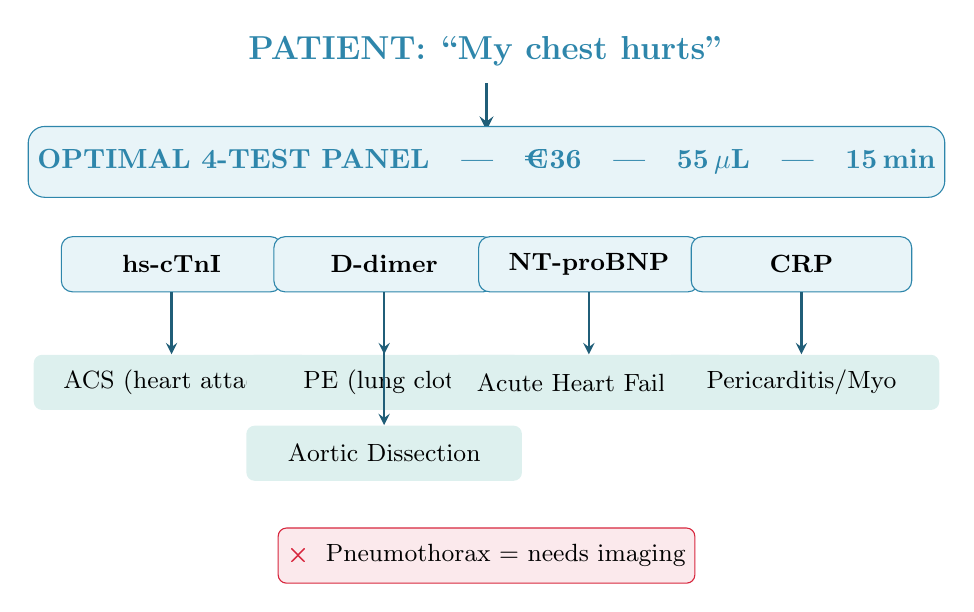
\begin{tikzpicture}[
  every node/.style={font=\small},
  test/.style={draw=accent, fill=highlight, rounded corners=4pt,
    minimum width=2.8cm, minimum height=0.7cm, align=center, font=\small\bfseries},
  disease/.style={draw=none, fill=success!15, rounded corners=3pt,
    minimum width=3.5cm, minimum height=0.7cm, align=center, font=\small},
  uncov/.style={draw=alert, fill=alert!10, rounded corners=3pt,
    minimum width=3.5cm, minimum height=0.7cm, align=center, font=\small},
  arrow/.style={->, >=stealth, thick, color=accent!70!black}
]

% Title
\node[font=\large\bfseries, color=accent] at (0, 4.2) {PATIENT: ``My chest hurts''};
\draw[arrow, very thick] (0, 3.8) -- (0, 3.2);

% Panel box
\node[draw=accent, fill=highlight, rounded corners=6pt,
  minimum width=11cm, minimum height=0.9cm, font=\bfseries\color{accent}]
  at (0, 2.8) {OPTIMAL 4-TEST PANEL\quad|\quad\texteuro36\quad|\quad55\,$\mu$L\quad|\quad15\,min};

% Tests
\node[test] (t1) at (-4, 1.5) {hs-cTnI};
\node[test] (t2) at (-1.3, 1.5) {D-dimer};
\node[test] (t3) at (1.3, 1.5) {NT-proBNP};
\node[test] (t4) at (4, 1.5) {CRP};

% Diseases
\node[disease] (d1) at (-4, 0) {ACS (heart attack)};
\node[disease] (d2) at (-1.3, 0) {PE (lung clot)};
\node[disease] (d3) at (-1.3, -0.9) {Aortic Dissection};
\node[disease] (d4) at (1.3, 0) {Acute Heart Failure};
\node[disease] (d5) at (4, 0) {Pericarditis/Myo};
\node[uncov]   (d6) at (0, -2.2) {\textcolor{alert}{\textbf{\texttimes}}\; Pneumothorax = needs imaging};

% Arrows
\draw[arrow] (t1) -- (d1);
\draw[arrow] (t2) -- (d2);
\draw[arrow] (t2) -- (d3);
\draw[arrow] (t3) -- (d4);
\draw[arrow] (t4) -- (d5);

\end{tikzpicture}
\end{center}


% ══════════════════════════════════════════════════════════════════════════════
\section{Key Terminology}

\begin{table}[h]
\centering\small
\renewcommand{\arraystretch}{1.25}
\begin{tabular}{@{}p{3.2cm}p{11cm}@{}}
\toprule
\textbf{Term} & \textbf{Meaning} \\
\midrule
Sensitivity & Probability the test is positive when the disease is truly present (higher = better at detecting) \\
Specificity & Probability the test is negative when the disease is truly absent (\emph{not modelled here}) \\
$\tau$ (tau) & The sensitivity threshold --- test must detect the disease at least this well to ``count'' (default: 0.90 = 90\%) \\
Coverage & Fraction of the 6 pathologies covered by at least one test above $\tau$ \\
MHS & Minimal Hitting Set --- smallest group that ``hits'' every target \\
Set Cover & Pick the fewest sets (tests) whose union covers the entire universe (diseases) \\
ILP & Integer Linear Program --- optimisation where variables are whole numbers (0 or 1 = include/exclude) \\
Pareto optimal & A solution where you can't improve one objective (e.g.\ cost) without worsening another (e.g.\ coverage) \\
Ablation & Removing one component and measuring the damage \\
Bootstrap & Randomly resample the data many times to test stability \\
POC & Point-of-care --- testing done at bedside/clinic, not sent to a central lab \\
\bottomrule
\end{tabular}
\end{table}


% ══════════════════════════════════════════════════════════════════════════════
\section{SISTER ACT Score: Closing the Gap}

The biomarker panel misses pneumothorax (no blood test works). The
\textbf{SISTER ACT score} fixes this by adding an \textbf{AI e-stethoscope}
--- a digital stethoscope with built-in machine learning that ``listens''
for absent breath sounds.

\begin{tcolorbox}[resultbox, title={SISTER ACT = S-I-S-T-E-R-ACT (0--20 points)}]
\begin{tabular}{@{}clcl@{}}
\textbf{S} & Symptoms        & 0--3 & Chest pain typicality, dyspnoea \\
\textbf{I} & Imaging (AI e-stethoscope) & 0--3 & Absent sounds (PTX), crackles (HF), rub \\
\textbf{S} & Signs           & 0--2 & JVD, leg swelling, asymmetric BP \\
\textbf{T} & Timeline        & 0--3 & $<2$h = serial troponin needed \\
\textbf{E} & ECG             & 0--3 & ST changes, RBBB, S1Q3T3 \\
\textbf{R} & Risk factors    & 0--3 & Age $>65$, prior CVD, immobilisation \\
\textbf{ACT} & Acute Chemistry Testing & 0--3 & POC biomarker results \\
\end{tabular}
\end{tcolorbox}

\begin{tcolorbox}[alertbox, title={Three Tiers}]
\textbf{Low (0--6):} Discharge with safety-netting \quad
\textbf{Moderate (7--13):} POC serial testing \quad
\textbf{High (14--20):} Immediate referral
\end{tcolorbox}

\subsection{Simulation Results ($n = 10{,}000$)}

\begin{table}[h]
\centering\small
\begin{tabular}{@{}lrrr@{}}
\toprule
\textbf{Metric} & \textbf{HEAR} & \textbf{HEART} & \textbf{SISTER ACT} \\
\midrule
Sensitivity         & 96.0\% & 97.7\% & \textbf{97.7\%} \\
Specificity         & 42.4\% & 49.3\% & \textbf{70.0\%} \\
NPV (low tier)      & .987   & .994   & \textbf{.996} \\
Missed per 1{,}000  & 4.8    & 2.8    & \textbf{2.8} \\
Referral rate       & 62.2\% & 56.4\% & \textbf{38.2\%} \\
PTX sensitivity     & 93.9\% & 91.8\% & \textbf{95.9\%} \\
Pathologies covered & 6/6    & 6/6    & \textbf{6/6} \\
\bottomrule
\end{tabular}
\end{table}

\begin{tcolorbox}[resultbox, title={Key Numbers}]
\textbf{Coverage:} 5/6 (biomarker only) $\to$ \textbf{6/6} (+AI e-stethoscope) \\
\textbf{Marginal cost:} \texteuro0.64/patient (device amortised over 3 years) \\
\textbf{PTX detection:} 14\% $\to$ \textbf{96\%} (+82 pp) \\
\textbf{Referral reduction:} $-$24 pp vs HEAR, $-$18 pp vs HEART
\end{tcolorbox}


% ══════════════════════════════════════════════════════════════════════════════
\section{The Big Insight}

\begin{tcolorbox}[insightbox, title={Take-home message}]
Single-axis testing (one test for one disease) is how we've always done it.
But chest pain has 6 possible causes. By borrowing a math trick from cancer
drug design, we can find the optimal multi-disease panel with just
\textbf{4 cheap, fast, fingerprick blood tests}.

This is the same as asking: ``What is the minimum number of antibiotics to
cover every possible bacterial strain?'' --- a \textbf{covering problem}.
\end{tcolorbox}


% ══════════════════════════════════════════════════════════════════════════════
\section{What This Paper Does NOT Do}

\begin{itemize}[nosep]
  \item[\textcolor{alert}{\texttimes}] Does NOT use any new patient data ---
    everything comes from published studies
  \item[\textcolor{success}{\checkmark}] \textbf{Does} model specificity, PPV/NPV, and panel-level false-positive rate (93.4\%)
  \item[\textcolor{success}{\checkmark}] \textbf{Does} model serial testing (ESC 0/1h and 0/3h troponin protocols) and time-dependent kinetics
  \item[\textcolor{alert}{\texttimes}] Does NOT account for correlations
    between tests in the same patient
  \item[\textcolor{alert}{\texttimes}] Does NOT claim the panel is clinically
    validated --- it is a hypothesis to be tested in the SISTER ACT trial
\end{itemize}

\end{document}
